\subsubsection{Data collection \& management}

We have developed an innovative platform for housing of mice in large arenas
(\textgreater 2m diameter) enabling precise behavioural manipulation and
high-resolution monitoring [Figure~\ref{fig:arena}, \cite{campagnerEtAl24}].
%
We have openly shared software for supporting data acquisition
[\cite{aeonacquisition}] and management [\cite{aeonmecha}] in this
arena.
%
Additionally, the platforms supports continuous, long term monitoring of neural
activity with Neuropixels probes, capable of recording from thousands of
neurons simultaneously spanning the entire brain depth.
%
This setup has allowed us to collect several week-long datasets with single and
multiple mice per arena.

To facilitate the replication of our experimental setup by other groups, we
will share instructions for building foraging arenas, as well as specifications
of hardware used in them,
%
and we will improve the documentation of the software repositories for data
acquisition and management.


\begin{figure}
    \centering
    \subfloat[]{
        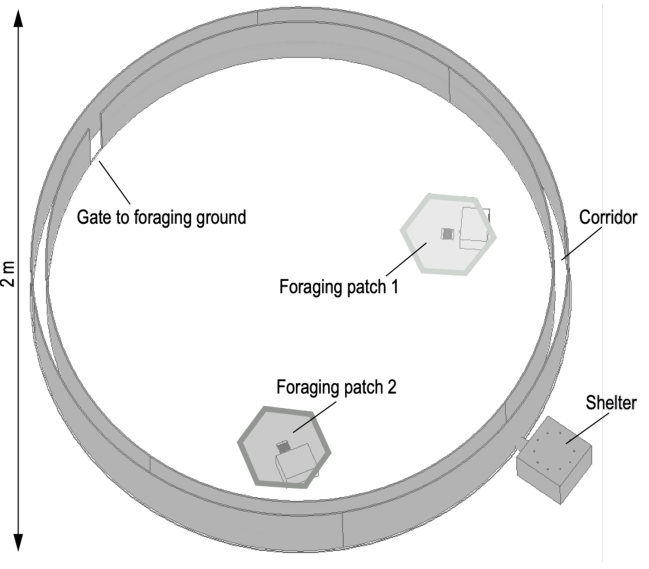
\includegraphics[width=4in]{figures/arena.png}
    }
    \hfill
    \subfloat[]{
        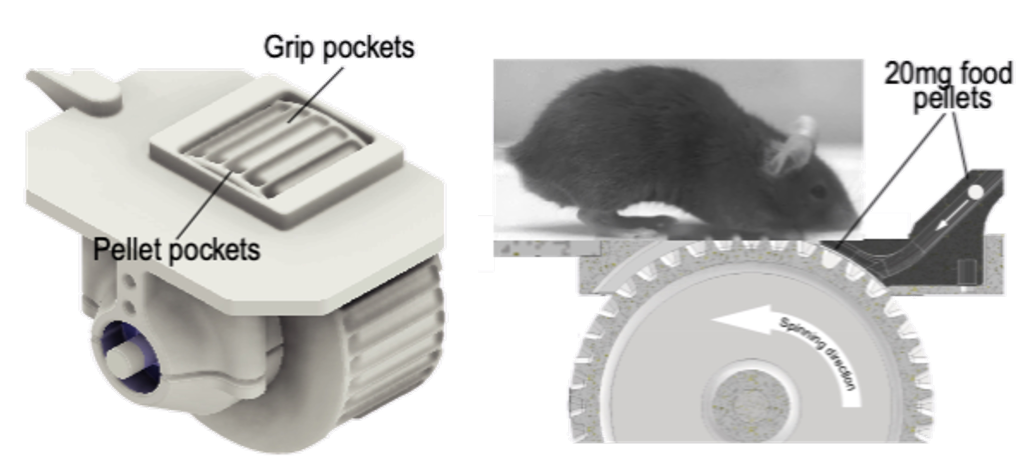
\includegraphics[width=4in]{figures/patch.png}
    }
    \caption{Foraging Arena (a) and Feeder (b).
    %
    The arena is composed of tessellated hexagonal tiles (a), each featuring a
    newly designed underground feeder (b).
    %
    Pellets are dispensed onto a foraging wheel once the mouse has spun it for
    a pre-defined programmable distance threshold using its forepaws (fictive
    digging).
    %
    The arena contains up to six scale-equipped nesting modules that allows
    housing of mice in the arena and weight monitoring.
    %
    Behavioural monitoring is achieved by an array of high-speed cameras (up to
    15), by which mouse location, mouse identity and body parts can be track in
    real time.
    %
    }
\label{fig:arena}
\end{figure}


\subsubsection{Sharing data and methods}

The very large datasets produced by NaLoDuCo experiments make traditional
methods of data distribution impractical. Instead, users will interact with the
data directly where it is stored. The maturation of cloud technologies now
makes this possible.

We will leverage the Distributed Archives for Neuroscience Data Integration
(DANDI), which utilises Amazon S3 storage, for hosting the data. Additionally,
we will provide software to visualise and analyse data using Amazon EC2
instances, thereby minimising the need for time-consuming data transfers.

Handling and sharing continuous behavioural and neural recordings of this scale
presents unique challenges. Runtime performance is one of them. If we
encounter unacceptable delays, we will explore advanced optimisation
strategies, such as parallel processing and resource-efficient cloud
configurations.

\subsubsection{Data visualisation}

Our visualisation tools
need to display very large datasets at different temporal scales, from
milliseconds to weeks and months, and they need to be web based.
%
We will use multi-resolution visualisation techniques, which store data at
various resolutions, and use the appropriate resolution for each zoom level.
%
Web-based visualisation will be optimised using web workers
[\cite{webWorkers}].

\subsubsection{Spike sorting}

Spike sorting is specially challenging in NaLoDuCo experimentation since we
want to track individual neurons of freely moving mice for weeks to months.
%
In addition, we need online spike sorting, to allow experiments driven
by real-time machine learning inference, as described below.
%
We will evaluate methods for tracking neurons over long periods of time
[e.g., \cite{yuanEtAl24,vanBeestEtAl24}] and for online sorting
[e.g., \cite{rutishauserEtAl06,santhanamEtAl04}]. If needed, we will develop
new methods, as we have experience on the subject~[\cite{sahani99}].

\subsubsection{Data analysis}

The very large size of NaLoDuCo experimental data, the fact that the statistics
of these data change across time, and the requirement for real-time and
close-loop inference create new challenges to conventional machine learning
data analysis methods.
%
We will evaluate existing methods targeting the experimental problems
in Figure~\ref{fig:dataAnalysis} and, if necessary, modify them, or create new
ones, to address the previous challenges.

For behavioural data, we will evaluate methods to:

\begin{itemize}

    \item track multiple body parts of
animals [e.g., \cite{mathisEtAl18,pereiraEtAl22,bidermanEtAl24} and a switching-linear-dynamical method using RFIDs that
we will develop],

    \item infer kinematics of foraging mice [e.g.,
        \cite{ldspython,challaEtAl11}],

    \item segment behaviour into discrete states [e.g., \cite{wiltschkoEtAl15,hsuAndYttri21} and a hierarchical HMM
that we will develop],

    \item infer the rules that govern mice behaviour from behavioural observations
        only (i.e., policy inference) [e.g., \cite{ziebartEtAl08,zhuEtAl23}].

\end{itemize}

For neural data, we will evaluate methods to:

\begin{itemize}

    \item estimate low-dimensional continual representations of
        neural activity (i.e., latents inference)
        [e.g.,
        \cite{mackeEtAl11,dunckerAndSahani18,walkerEtAl23,pandarinathEtAl18,saniEtAl21}],

    \item segment neural activity into discrete states
        [e.g., \cite{chenEtAl09,escolaEtAl11}],

    \item decode environment variables from neural activity
        [e.g., \cite{dengEtAl15,kloostermanEtAl14,tampuuEtAl19}].

\end{itemize}


\subsubsection{Inference-driven experimentation}

We call inference-driven experimentation to a type of experimentation driven by
machine learning inferences on neural or behavioural data, where the result of
these inferences can change the experiment in real time.

We will apply inference-driven experimentation to test if patterns of neural
activity are causally related to foraging behaviours.
%
We would first check that a pattern of neural activity always precedes a given
foraging behaviour. We would then detect the occurrence of the pattern and in
real time optogenetically inactivate the neurons responsible for the pattern.
%
If the behaviour disappears the causality argument would be supported.

For this we will use the Bonsai ecosystem for experimental
control~\cite{bonsai} and online machine learning functionality that we are
adding to Bonsai~\cite{bonsaiML}, funded by a BBSRC award~\cite{bbsrcAward}.

